\documentclass[12pt]{article}
\usepackage[top=1in]{geometry}
\usepackage{graphicx}
\usepackage{amsmath}    % need for subequations
\usepackage{graphicx}   % need for figures
\usepackage{verbatim}   % useful for program listings
\usepackage{color}      % use if color is used in text
\usepackage{amsthm}
\usepackage{amsfonts}
\usepackage{amssymb}
\usepackage{subfigure}  % use for side-by-side figures
\usepackage[hidelinks]{hyperref}   % use for hypertext links, including those to external documents and URLs
\usepackage{algorithmic}
\usepackage{listings}
\usepackage[linesnumbered,ruled,vlined,commentsnumbered]{algorithm2e}
\usepackage[export]{adjustbox}
\usepackage{changepage}
\usepackage{parallel}
\usepackage{float}
\usepackage{xcolor}
\usepackage{caption}
%\usepackage{subcaption}

\newtheorem*{conjecture}{Conjecture}


\begin{document}

\begin{center}
 
{\bf\large The 21\textemdash or only 16\textemdash Holdout Classes Among Skelet's\\ 43 Hardly Non-Regular Turing Machines} \\
 
       %\vspace{0.5cm}
 
 
       \textbf{Daniel Briggs}
              %\vspace{0.5cm}


\end{center}

%\begin{abstract}
%\end{abstract}

\section*{Introduction}
In 2003, Skelet (Georgi Georgiev) released a 6218-line uncommented Pascal program ``bbfind'' that goes through the approximately 150 million (by the program's count) essentially distinct 5-state Turing machines and for each one attempts to either prove that it never halts when run on a blank tape or run it until it does. After a run of about two weeks, only 164 machines had stumped the program. Of these, 54 began with writing 0 to the tape, and so their runs were equivalent with an offset in number of steps to machines among the other 110. These 110 machines included 67 which were found to be ``shift recursive'' and so easily provable never to halt by hand.

Skelet dubbed the 43 remaining machines ``Hardly non-regular,'' and although his work has never been independently verified, his list has remained the starting point for anyone interested in finishing the Busy Beaver of 5 ever since.

The 27th of these 43 machines was classified as ``BL\_2'' by Skelet, and the other 42 were not classified. Note that for this reason, the machines I refer to as \#s 28\textendash43 are often referred to as 27\textendash42 by other authors\textemdash including myself, previously.

From this list of 43, \#2, \#5, and \#6 are equivalent with an offset in step number, \#13 is equivalent to \#12,  \#29 is equivalent to \#23, \#s 21, 28, and 39 are equivalent with an offset,  and \#41 is equivalent with an offset to \#30; thus we are left with 36 essentially distinct Turing machines to study.

Of these 36, \#s 16, 24, and 38 reach a phase (of at least 1 trillion steps) of equivalent action with an offset, but with several bits beyond what seems to be the working tape that are different; thus they have not been proved equivalent, but deserve to be talked about together. The situation is the same with machines \#19 \& \#42. So instead of 36 machines, we talk of 33 different studies to be made.

Of these, I (and others independently) have discovered that machines 2 (and so 5 and 6), 14, 18, and 25 are trivially proved never to halt. I also proved machines \#8, \#9, \#10, \#11, and \#12 (and so \#13) never to halt. Machines \#21 (and so \#28 and \#39), \#31 and \#32 were proved by univerz (Pavel Kropitz). univerz in fact showed the non-halting of twelve machines, but we need only reference these three for our reduction in number.

Thus there are 21 studies that need to be performed; thus this document is organized into 21 sections.

Machine \#4 was seen to be trivial and \#s 20 and 23 easy if arduous in the course of producing this document,
and machine classes $16\sim24\sim38$ and $19\sim42$ require but a simple proof as well.

\texttt{\href{https://github.com/danbriggs/Turing/blob/master/doc/record7-19-20.txt}
{github.com/danbriggs/Turing/blob/master/doc/record7-19-20.txt}}
is where the reader is encouraged to go to get the state diagrams for the machines.

\newpage
\tableofcontents
\clearpage
\phantomsection
\addcontentsline{toc}{section}{1}
\section*{1}
\clearpage
\phantomsection
\addcontentsline{toc}{section}{3}
\section*{3}
The cleanest way to study HNR\#3 is probably to inspect moments when the tape head is on the right; at these moments, the whole tape tends to be comprised of long runs of 1s with just a very few isolated 0s\textemdash often just one 0\textemdash in between. Ignoring step numbers when the tape head is on the right after it had also recently\textemdash within the past 10 steps\textemdash been at the right, we find that it achieves this configuration in state A with bit 1, state C with bit 1, state D with bit 1, or state C with bit 0\textemdash these results are for when the machine has reached the rightmost bit of the swath ever accessed, not just the current nonzero swath.

When it is in state A and there is only one 0 in between, it seems that both swaths of 1s, excluding the 1 at the tape head, may always be of even length. In order to get a handle on what it does by the time it reaches the right again afterwards, after leaving the right for at least 10 steps, I simulated runs starting from this type of configuration with two swaths of 1s of all possible even lengths up to 118, and recorded how many steps it took to get back to the right, how many swaths of 1s there were afterwards, how long the leftmost and rightmost of these were, and what state it ended up in\textemdash this time, ``on the right'' meaning at the rightmost 1. Tables \ref{tab:3nums}, \ref{tab:3swaths}, \ref{tab:3states}, \ref{tab:3lefts}, and \ref{tab:3rights} give this data for swaths of 1s of even length $\leq28$; Table \ref{tab:3steps} shows moments when the tape head is on the right when started on a blank tape.

\begin{small}
\begin{table}[H]
\begin{adjustwidth}{-1.5cm}{-1.5cm}
\texttt{
\begin{tabular}{ccccccccccccccc}
43&51&85&93&133&141&187&195&247&255&313&321&385&393&463\\
27&33&39&45&51&57&63&69&75&81&87&93&99&105&111\\
119&171&179&237&245&309&317&387&395&471&479&561&569&657&665\\
63&69&75&81&87&93&99&105&111&117&123&129&135&141&147\\
273&279&285&291&297&303&309&315&321&327&333&339&345&351&357\\
105&111&117&123&129&135&141&147&153&159&165&171&177&183&189\\
275&345&353&429&437&519&527&615&623&717&725&825&833&939&947\\
153&159&165&171&177&183&189&195&201&207&213&219&225&231&237\\
527&579&587&645&653&717&725&795&803&879&887&969&977&1065&1073\\
207&213&219&225&231&237&243&249&255&261&267&273&279&285&291\\
461&549&557&651&659&759&767&873&881&993&1001&1119&1127&1251&1259\\
267&273&279&285&291&297&303&309&315&321&327&333&339&345&351\\
849&855&861&867&873&879&885&891&897&903&909&915&921&927&933\\
333&339&345&351&357&363&369&375&381&387&393&399&405&411&417\\
677&783&791&903&911&1029&1037&1161&1169&1299&1307&1443&1451&1593&1601\\
\end{tabular}
}
\end{adjustwidth}
\caption{\label{tab:3nums}Number of steps taken to once again arrive at the rightmost 1 bit after leaving for at least 10 steps starting with configuration $1^{2m}01^{2n}i~A$ for $0\leq m,n\leq14$. Here $m$ is the row number and $n$ is the column number, both indexed from 0.}
\end{table}
\end{small}

\begin{small}
\begin{table}[H]
\texttt{
\begin{tabular}{ccccccccccccccc}
2&2&2&2&2&2&2&2&2&2&2&2&2&2&2\\
1&1&1&1&1&1&1&1&1&1&1&1&1&1&1\\
2&2&2&2&2&2&2&2&2&2&2&2&2&2&2\\
2&2&2&2&2&2&2&2&2&2&2&2&2&2&2\\
3&3&3&3&3&3&3&3&3&3&3&3&3&3&3\\
2&2&2&2&2&2&2&2&2&2&2&2&2&2&2\\
2&2&2&2&2&2&2&2&2&2&2&2&2&2&2\\
2&2&2&2&2&2&2&2&2&2&2&2&2&2&2\\
3&3&3&3&3&3&3&3&3&3&3&3&3&3&3\\
2&2&2&2&2&2&2&2&2&2&2&2&2&2&2\\
2&2&2&2&2&2&2&2&2&2&2&2&2&2&2\\
2&2&2&2&2&2&2&2&2&2&2&2&2&2&2\\
3&3&3&3&3&3&3&3&3&3&3&3&3&3&3\\
2&2&2&2&2&2&2&2&2&2&2&2&2&2&2\\
2&2&2&2&2&2&2&2&2&2&2&2&2&2&2\\
\end{tabular}}
\caption{\label{tab:3swaths}Number of swaths of 1s produced upon arriving at the rightmost 1 bit after leaving for at least 10 steps starting with configuration $1^{2m}01^{2n}i~A$ for $0\leq m,n\leq14$. Here $m$ is the row number and $n$ is the column number; both are indexed from 0. Note there seems to be no dependence on the number of 1s to the right of the 0.}
\end{table}
\end{small}

\begin{small}
\begin{table}[H]
\texttt{
\begin{tabular}{ccccccccccccccc}
A&C&A&C&A&C&A&C&A&C&A&C&A&C&A\\
D&D&D&D&D&D&D&D&D&D&D&D&D&D&D\\
C&A&C&A&C&A&C&A&C&A&C&A&C&A&C\\
D&D&D&D&D&D&D&D&D&D&D&D&D&D&D\\
D&D&D&D&D&D&D&D&D&D&D&D&D&D&D\\
D&D&D&D&D&D&D&D&D&D&D&D&D&D&D\\
C&A&C&A&C&A&C&A&C&A&C&A&C&A&C\\
D&D&D&D&D&D&D&D&D&D&D&D&D&D&D\\
C&A&C&A&C&A&C&A&C&A&C&A&C&A&C\\
D&D&D&D&D&D&D&D&D&D&D&D&D&D&D\\
C&A&C&A&C&A&C&A&C&A&C&A&C&A&C\\
D&D&D&D&D&D&D&D&D&D&D&D&D&D&D\\
D&D&D&D&D&D&D&D&D&D&D&D&D&D&D\\
D&D&D&D&D&D&D&D&D&D&D&D&D&D&D\\
C&A&C&A&C&A&C&A&C&A&C&A&C&A&C\\
\end{tabular}}
\caption{\label{tab:3states}State of the machine upon arriving at the rightmost 1 bit after leaving for at least 10 steps starting with configuration $1^{2m}01^{2n}i~A$ for $0\leq m,n\leq14$. Here $m$ is the row number and $n$ is the column number, both indexed from 0.}
\end{table}
\end{small}

\begin{small}
\begin{table}[H]
\texttt{
\begin{tabular}{ccccccccccccccc}
2&2&4&4&6&6&8&8&10&10&12&12&14&14&16\\
10&12&14&16&18&20&22&24&26&28&30&32&34&36&38\\
2&4&4&6&6&8&8&10&10&12&12&14&14&16&16\\
2&2&2&2&2&2&2&2&2&2&2&2&2&2&2\\
4&4&4&4&4&4&4&4&4&4&4&4&4&4&4\\
4&4&4&4&4&4&4&4&4&4&4&4&4&4&4\\
4&6&6&8&8&10&10&12&12&14&14&16&16&18&18\\
6&6&6&6&6&6&6&6&6&6&6&6&6&6&6\\
4&4&4&4&4&4&4&4&4&4&4&4&4&4&4\\
8&8&8&8&8&8&8&8&8&8&8&8&8&8&8\\
6&8&8&10&10&12&12&14&14&16&16&18&18&20&20\\
10&10&10&10&10&10&10&10&10&10&10&10&10&10&10\\
10&10&10&10&10&10&10&10&10&10&10&10&10&10&10\\
12&12&12&12&12&12&12&12&12&12&12&12&12&12&12\\
8&10&10&12&12&14&14&16&16&18&18&20&20&22&22\\
\end{tabular}}
\caption{\label{tab:3lefts}Length of the leftmost swath of 1s produced upon arriving at the rightmost 1 bit after leaving for at least 10 steps starting with configuration $1^{2m}01^{2n}i~A$ for $0\leq m,n\leq14$. Here $m$ is the row number and $n$ is the column number, both indexed from 0.}
\end{table}
\end{small}

\begin{small}
\begin{table}[H]
\texttt{
\begin{tabular}{ccccccccccccccc}
5&7&7&9&9&11&11&13&13&15&15&17&17&19&19\\
10&12&14&16&18&20&22&24&26&28&30&32&34&36&38\\
13&13&15&15&17&17&19&19&21&21&23&23&25&25&27\\
12&14&16&18&20&22&24&26&28&30&32&34&36&38&40\\
4&6&8&10&12&14&16&18&20&22&24&26&28&30&32\\
14&16&18&20&22&24&26&28&30&32&34&36&38&40&42\\
19&19&21&21&23&23&25&25&27&27&29&29&31&31&33\\
16&18&20&22&24&26&28&30&32&34&36&38&40&42&44\\
13&13&15&15&17&17&19&19&21&21&23&23&25&25&27\\
18&20&22&24&26&28&30&32&34&36&38&40&42&44&46\\
25&25&27&27&29&29&31&31&33&33&35&35&37&37&39\\
20&22&24&26&28&30&32&34&36&38&40&42&44&46&48\\
4&6&8&10&12&14&16&18&20&22&24&26&28&30&32\\
22&24&26&28&30&32&34&36&38&40&42&44&46&48&50\\
31&31&33&33&35&35&37&37&39&39&41&41&43&43&45\\
\end{tabular}}
\caption{\label{tab:3rights}Length of the rightmost swath of 1s produced upon arriving at the rightmost 1 bit after leaving for at least 10 steps starting with configuration $1^{2m}01^{2n}i~A$ for $0\leq m,n\leq14$. Here $m$ is the row number and $n$ is the column number, both indexed from 0.}
\end{table}
\end{small}

\begin{small}
\begin{table}[H]
\begin{Parallel}[c]{0.48\textwidth}{0.48\textwidth}
\ParallelLText{
\texttt{
\begin{tabular}{rcccl}
43&A&1&6&$1^{2}01^{4}i$\\
83&D&0&13&$1^{13}i$\\
268&A&1&18&$1^{8}01^{10}i$\\
572&D&2&30&$1^{4}01^{13}01^{13}i$\\
923&A&1&34&$1^{14}01^{20}i$\\
1137&D&1&41&$1^{6}01^{35}i$\\
1300&D&1&47&$1^{2}01^{45}i$\\
1457&D&0&53&$1^{53}i$\\
2512&A&1&58&$1^{28}01^{30}i$\\
4262&A&1&68&$1^{24}01^{44}i$\\
5244&D&2&80&$1^{10}01^{23}01^{47}i$\\
6881&C&1&84&$1^{36}01^{48}i$\\
7035&C&1&84&$1^{38}01^{46}o$\\
7731&D&1&89&$1^{18}01^{71}i$\\
8146&D&1&95&$1^{8}01^{87}i$\\
8675&D&2&106&$1^{4}01^{13}01^{89}i$\\
11762&A&1&110&$1^{52}01^{58}i$\\
16410&A&1&120&$1^{44}01^{76}i$\\
21486&C&1&130&$1^{50}01^{80}i$\\
21736&C&1&130&$1^{52}01^{78}o$\\
27456&C&1&138&$1^{52}01^{86}i$\\
27724&C&1&138&$1^{54}01^{84}o$\\
28930&D&1&143&$1^{26}01^{117}i$\\
29609&D&1&149&$1^{12}01^{137}i$\\
35900&C&1&158&$1^{72}01^{86}i$\\
36168&C&1&158&$1^{74}01^{84}o$\\
38004&D&1&163&$1^{36}01^{127}i$\\
46117&A&1&172&$1^{74}01^{98}i$\\
48005&D&1&179&$1^{36}01^{143}i$\\
57450&A&1&188&$1^{82}01^{106}i$\\
59656&D&1&195&$1^{40}01^{155}i$\\
61763&D&2&206&$1^{16}01^{33}01^{157}i$\\
71594&A&1&210&$1^{98}01^{112}i$\\
74478&D&1&217&$1^{48}01^{169}i$\\
86025&C&2&231&$1^{10}01^{109}01^{112}i$\\
86371&C&2&231&$1^{10}01^{111}01^{110}o$\\
99063&A&1&234&$1^{68}01^{166}i$\\
\end{tabular}}}
\ParallelRText{
\texttt{
\begin{tabular}{rcccl}
114997&A&1&244&$1^{102}01^{142}i$\\
118151&D&1&251&$1^{50}01^{201}i$\\
119604&D&1&257&$1^{24}01^{233}i$\\
121147&D&2&268&$1^{10}01^{23}01^{235}i$\\
137166&C&1&272&$1^{130}01^{142}i$\\
137602&C&1&272&$1^{132}01^{140}o$\\
159556&A&1&280&$1^{104}01^{176}i$\\
167144&D&2&292&$1^{40}01^{73}01^{179}i$\\
184393&C&1&296&$1^{132}01^{164}i$\\
184895&C&1&296&$1^{134}01^{162}o$\\
189755&D&1&301&$1^{66}01^{235}i$\\
191778&D&1&307&$1^{32}01^{275}i$\\
193873&D&3&323&$1^{4}01^{23}01^{19}01^{277}i$\\
214312&A&2&327&$1^{4}01^{165}01^{158}i$\\
240390&C&1&332&$1^{86}01^{246}i$\\
241138&C&1&332&$1^{88}01^{244}o$\\
247234&D&2&342&$1^{34}01^{63}01^{245}i$\\
272173&A&1&346&$1^{160}01^{186}i$\\
286901&D&3&363&$1^{16}01^{75}01^{83}01^{189}i$\\
307178&A&2&367&$1^{16}01^{173}01^{178}i$\\
338230&C&1&372&$1^{108}01^{264}i$\\
339032&C&1&372&$1^{110}01^{262}o$\\
342914&D&1&377&$1^{54}01^{323}i$\\
344841&D&1&383&$1^{26}01^{357}i$\\
346240&D&1&389&$1^{12}01^{377}i$\\
380071&C&1&398&$1^{192}01^{206}i$\\
380699&C&1&398&$1^{194}01^{204}o$\\
389825&D&1&403&$1^{96}01^{307}i$\\
396816&D&3&419&$1^{10}01^{49}01^{51}01^{309}i$\\
429039&A&2&423&$1^{10}01^{207}01^{206}i$\\
471335&C&1&428&$1^{116}01^{312}i$\\
472281&C&1&428&$1^{118}01^{310}o$\\
476709&D&1&433&$1^{58}01^{375}i$\\
478906&D&1&439&$1^{28}01^{411}i$\\
522833&A&1&448&$1^{214}01^{234}i$\\
533739&D&1&455&$1^{106}01^{349}i$\\
537694&D&1&461&$1^{52}01^{409}i$\\
\end{tabular}}}
\end{Parallel}
\caption{\label{tab:3steps}The step numbers when the tape head was at the rightmost bit of the swath ever accessed after leaving the right for at least 10 steps; what state the machine was in; how many intermediate zeros there were; how many 1s there were other than at the tape head; what the tape looked like. Run started on a blank tape.}
\end{table}
\end{small}

\newpage
Repeating the analysis done in Tables \ref{tab:3nums}, \ref{tab:3swaths}, \ref{tab:3states}, \ref{tab:3lefts}, and \ref{tab:3rights}, but with the machine starting in state C instead of A gives much simpler data: there are always two swaths; the number of steps and lengths of the left and right swaths are linear functions of the lengths of the original swaths; the machine ends up in state D as long as the right swath has at least six 1s. The machine starting in state D is exactly analogous to starting in state A, but the tape head is one bit further to the right and the step number is advanced by three. C with tape head at a 0 bit always comes from D with tape head at a 1 bit but otherwise of the same form.

Thus, it would suffice to understand the patterns shown in Tables \ref{tab:3nums}, \ref{tab:3swaths}, \ref{tab:3states}, \ref{tab:3lefts}, and \ref{tab:3rights} to predict the action of HNR\#3 from situations consisting of at most two swaths of 1s. However, situations with more than two swaths as shown in Table \ref{tab:3steps} may have to be understood separately, and could increase the difficulty of showing that HNR\#3 never halts or accelerating it until it does.

Out of the first billion steps, the maximum number of swaths of 1s when the tape head is on the right is 6, and this first occurs at step 6333029, when the machine is in state D, and the tape is \texttt{$1^4~0~1^{23}~0~1^{53}~0~1^{197}~0~1^{259}~0~1^{550}$}.

An argument backtracking from a halt state may be capable of sidestepping all this detailed analysis; it is clear from the machine diagram
\begin{table}[H]
\texttt{\begin{tabular}{rccccc}
&A&B&C&D&E\\
0&C1L&H1L&D1R&A1R&C0L\\
1&A0R&E1L&B0L&C1R&D1L
\end{tabular}}
\label{tab:HNR3}
\end{table}
\noindent that 01o A and 01o E are the only ways to achieve halting; these must come from 0o0 D, 010i B, respectively; the former is a dead-end, whereas the latter comes from 0101i C; unfortunately, this branches into three possibilities: 01011o A, 010o1 D, and 01011o E. These respectively come from 0101o0 D, 0100i E, and 010110i B; these, from 010i00 C, 01001i B, and 0101101i C;



\clearpage
\phantomsection
\addcontentsline{toc}{section}{4}
\section*{4}

Machine 4 seems to be a trivial one, the proof just needs to be carried out. It counts up in binary using 11 as 0 and 10 as 1, with less significant digits to the left, on the left side of the tape, with an additional o11 at the left end in C. Then after a number of steps increasing by a constant difference of 12 modified by four times the location in the number of the 0 to be turned into a 1 (increasing when that bit is \emph{closer}), it produces the next number, written in the same binary scheme, with an extra 0 as padding on the right before its bookend 011. For example,

\begin{small}
\begin{table}[H]
\texttt{
\begin{tabular}{rcrcl}
882&  C&           o1110101110111111111111111011& 11.& Then after 145,\\
1027& C&         o111111101011111111111111111011& 12.& Then after 165 (+20 3/1),\\
1192& C&       o11101110101111111111111111111011& 13.& Then after 173 (+8 1/2),\\
1365& C&     o1111101010111111111111111111111011& 14.& Then after 189 (+16 2/1),\\
1554& C&   o111010101011111111111111111111111011& 15.& Then after 185 (-4 1/5),\\
1739& C& o11111111111011111111111111111111111011& 16.& Then after 213 (+28).
\end{tabular}}
\caption{\label{tab:4}Machine 4. The numbers before and after the slash portray which bit in is to be turned from a 0 to a 1 previously/currently. The difference between the two numbers determines the multiple of 4 offset from 12 more the step difference will be above the previous step difference.}
\end{table}
\end{small}

\phantomsection
\addcontentsline{toc}{section}{7}
\section*{7}

\begin{small}
\begin{table}[H]
\begin{Parallel}[c]{0.48\textwidth}{0.48\textwidth}
\ParallelLText{
\texttt{
\begin{tabular}{rcr}
33&A&$1^{2}0^{1}1^{2}$\\
57&C&$1^{10}$\\
188&D&$1^{9}0^{1}1^{6}$\\
276&C&$1^{20}0^{1}1^{2}$\\
355&C&$1^{28}$\\
746&A&$1^{19}0^{1}1^{14}$\\
810&A&$1^{16}0^{1}1^{16}$\\
1602&D&$1^{19}0^{1}1^{23}0^{1}1^{4}$\\
2234&A&$1^{35}0^{1}1^{16}$\\
2346&A&$1^{32}0^{1}1^{18}$\\
2640&C&$1^{48}0^{1}1^{8}$\\
3049&C&$1^{50}0^{1}1^{13}0^{1}1^{4}$\\
4426&D&$1^{39}0^{1}1^{32}$\\
5816&C&$1^{42}0^{1}1^{19}0^{1}1^{23}0^{1}1^{4}$\\
7139&D&$1^{41}0^{1}1^{47}0^{1}1^{4}$\\
9473&D&$1^{69}0^{1}1^{28}$\\
12905&A&$1^{65}0^{1}1^{42}$\\
13107&A&$1^{62}0^{1}1^{44}$\\
17183&A&$1^{73}0^{1}1^{42}$\\
17409&A&$1^{70}0^{1}1^{44}$\\
21971&A&$1^{77}0^{1}1^{46}$\\
22209&A&$1^{74}0^{1}1^{48}$\\
26915&A&$1^{65}0^{1}1^{61}0^{1}1^{10}$\\
27117&A&$1^{62}0^{1}1^{63}0^{1}1^{10}$\\
31493&D&$1^{95}0^{1}1^{44}$\\
37941&D&$1^{89}0^{1}1^{60}$\\
45261&A&$1^{99}0^{1}1^{60}$\\
45565&A&$1^{96}0^{1}1^{62}$\\
47041&C&$1^{134}0^{1}1^{30}$\\
47840&C&$1^{156}0^{1}1^{14}$\\
48453&C&$1^{170}0^{1}1^{6}$\\
49018&C&$1^{180}0^{1}1^{2}$\\
49577&C&$1^{188}$\\
57768&A&$1^{99}0^{1}1^{94}$\\
58072&A&$1^{96}0^{1}1^{96}$\\
64426&C&$1^{98}0^{1}1^{51}0^{1}1^{49}0^{1}1^{10}$\\
70891&D&$1^{101}0^{1}1^{101}0^{1}1^{10}$\\
81739&D&$1^{153}0^{1}1^{64}$\\
93763&A&$1^{113}0^{1}1^{97}0^{1}1^{23}0^{1}1^{4}$\\
94109&A&$1^{110}0^{1}1^{99}0^{1}1^{23}0^{1}1^{4}$\\
\end{tabular}}}
\ParallelRText{
\texttt{
\begin{tabular}{rcr}
105757&D&$1^{155}0^{1}1^{81}0^{1}1^{4}$\\
120999&A&$1^{161}0^{1}1^{84}$\\
121489&A&$1^{158}0^{1}1^{86}$\\
123997&C&$1^{208}0^{1}1^{42}$\\
125270&C&$1^{236}0^{1}1^{20}$\\
141651&D&$1^{141}0^{1}1^{124}$\\
162381&A&$1^{173}0^{1}1^{102}$\\
162907&A&$1^{170}0^{1}1^{104}$\\
170467&C&$1^{172}0^{1}1^{73}0^{1}1^{40}$\\
186702&A&$1^{161}0^{1}1^{128}$\\
187192&A&$1^{158}0^{1}1^{130}$\\
191812&C&$1^{230}0^{1}1^{64}$\\
211699&A&$1^{151}0^{1}1^{135}0^{1}1^{23}0^{1}1^{4}$\\
212159&A&$1^{148}0^{1}1^{137}0^{1}1^{23}0^{1}1^{4}$\\
232791&A&$1^{213}0^{1}1^{99}0^{1}1^{4}$\\
233437&A&$1^{210}0^{1}1^{101}0^{1}1^{4}$\\
259509&D&$1^{207}0^{1}1^{112}$\\
284371&D&$1^{163}0^{1}1^{149}0^{1}1^{22}$\\
309195&A&$1^{233}0^{1}1^{106}$\\
309901&A&$1^{230}0^{1}1^{108}$\\
340719&A&$1^{205}0^{1}1^{142}$\\
341341&A&$1^{202}0^{1}1^{144}$\\
370731&A&$1^{177}0^{1}1^{155}0^{1}1^{28}$\\
371269&A&$1^{174}0^{1}1^{157}0^{1}1^{28}$\\
399339&D&$1^{245}0^{1}1^{118}$\\
403579&C&$1^{312}0^{1}1^{58}$\\
405584&C&$1^{348}0^{1}1^{28}$\\
438615&D&$1^{203}0^{1}1^{182}$\\
446809&C&$1^{302}0^{1}1^{90}$\\
449912&C&$1^{354}0^{1}1^{44}$\\
487277&A&$1^{219}0^{1}1^{188}$\\
487941&A&$1^{216}0^{1}1^{190}$\\
496785&C&$1^{318}0^{1}1^{94}$\\
500104&C&$1^{372}0^{1}1^{46}$\\
501965&C&$1^{402}0^{1}1^{22}$\\
503430&C&$1^{420}0^{1}1^{10}$\\
504787&C&$1^{432}0^{1}1^{4}$\\
546044&D&$1^{227}0^{1}1^{218}$\\
557280&C&$1^{344}0^{1}1^{108}$\\
608971&D&$1^{261}0^{1}1^{200}$\\
\end{tabular}}}
\end{Parallel}
\caption{\label{tab:7}Machine 7, tapehead at leftmost bit. Perhaps analysis of HNR\#3 will serve HNR\#7 as well.}
\end{table}
\end{small}

\addcontentsline{toc}{section}{15}
\section*{15}

\begin{tiny}
\begin{table}[H]
\texttt{
\hspace*{-1.55in}
\setlength\tabcolsep{2pt}
\begin{tabular}{rrrrr}
31167&C&$i1^{0}0111111101011111110101011111010111010101011101111111010101010101011$&diff&off\\
31203&C&$i1^{4}01110101{\textcolor{red}{1}}1011111110101011111010111010101011101111111010101010101011$&+36&0\\
31267&C&$i1^{8}011101{\textcolor{red}{1}}111011111110101011111010111010101011101111111010101010101011$&+64&-8\\
31407&C&$i1^{12}0111011101{\textcolor{red}{1}}11111110101011111010111010101011101111111010101010101011$&+140&-4\\
31703&C&$i1^{16}011101110101010101{\textcolor{red}{1}}101011111010111010101011101111111010101010101011$&+296&8\\
32271&C&$i1^{20}011101110101{\textcolor{red}{1}}101011101011111010111010101011101111111010101010101011$&+568&-8\\
33415&C&$i1^{24}01110111010111{\textcolor{red}{1}}1011101011111010111010101011101111111010101010101011$&+1144&-8\\
35711&C&$i1^{28}0111011101011111{\textcolor{red}{1}}11101011111010111010101011101111111010101010101011$&+2296&-8\\
40315&C&$i1^{32}01110111010111111101{\textcolor{red}{1}}1011111010111010101011101111111010101010101011$&+4604&-4\\
49527&C&$i1^{36}0111011101011111110101{\textcolor{red}{1}}11111010111010101011101111111010101010101011$&+9212&-4\\
67963&C&$i1^{40}0111011101011111110101010101{\textcolor{red}{1}}10111010101011101111111010101010101011$&+18436&4\\
104819&C&$i1^{44}011101110101111111010101{\textcolor{red}{1}}101110111010101011101111111010101010101011$&+36856&-8\\
178539&C&$i1^{48}01110111010111111101010111{\textcolor{red}{1}}1110111010101011101111111010101010101011$&+73720&-8\\
325991&C&$i1^{52}011101110101111111010101111101{\textcolor{red}{1}}111010101011101111111010101010101011$&+147452&-4\\
620903&C&$i1^{56}0111011101011111110101011111010101{\textcolor{red}{1}}10101011101111111010101010101011$&+294912&0\\
1210719&C&$i1^{60}01110111010111111101010111110101{\textcolor{red}{1}}1110101011101111111010101010101011$&+589816&-8\\
2390363&C&$i1^{64}011101110101111111010101111101011101{\textcolor{red}{1}}101011101111111010101010101011$&+1179644&-4\\
4749655&C&$i1^{68}01110111010111111101010111110101110101{\textcolor{red}{1}}1011101111111010101010101011$&+2359292&-4\\
9468243&C&$i1^{72}0111011101011111110101011111010111010101{\textcolor{red}{1}}11101111111010101010101011$&+4718588&-4\\
18905427&C&$i1^{76}01110111010111111101010111110101110101010101{\textcolor{red}{1}}1111111010101010101011$&+9437184&0\\
37779787&C&$i1^{80}011101110101111111010101111101011101010101{\textcolor{red}{1}}111111111010101010101011$&+18874360&-8\\
75528531&C&$i1^{84}0111011101011111110101011111010111010101011101010101{\textcolor{red}{1}}10101010101011$&+37748744&8\\
151025995&C&$i1^{88}0111011101011111110101011111010111010101011101{\textcolor{red}{1}}10101110101010101011$&+75497464&-8\\
302020931&C&$i1^{92}011101110101111111010101111101011101010101110111{\textcolor{red}{1}}101110101010101011$&+150994936&-8\\
604010811&C&$i1^{96}01110111010111111101010111110101110101010111011111{\textcolor{red}{1}}1110101010101011$&+301989880&-8\\
1207990583&C&$i1^{100}011101110101111111010101111101011101010101110111111101{\textcolor{red}{1}}101010101011$&+603979772&-4\\
2415950131&C&$i1^{104}01110111010111111101010111110101110101010111011111110101{\textcolor{red}{1}}1010101011$&+1207959548&-4\\
4831869231&C&$i1^{108}0111011101011111110101011111010111010101011101111111010101{\textcolor{red}{1}}10101011$&+2415919100&-4\\
38654736675&C&$i1^{120}0111011101011111110101011111010111010101011101111111010101010101{\textcolor{red}{1}}11$&+19327352828&-4\\
\end{tabular}}
\caption{\label{tab:15}Machine 15. Let $i$ be the row in the table above, indexed from $-1$; let $x_i=36*2^{i}.$ Let $d_i$ be the
difference in step number between the $i$th row and the $i-1$st row, and let $k_i$ be the place of the first $1$ bit that was a
$0$ bit in the previous line, indexing from 0 just after the compressed portion. It is observed that $d_i-x_i$ relates to $k_i-2i$
in the following linear fashion: $d_i-x_i=-16+2(k_i-2i).$ Also, $k_i-2i$ always seems to be 2, 4, 6, 8, or 10. Also, the positions of the new
1s, highlighted in red, seem to be injective and surjective among every other position throughout the swath other than at the very end.
Furthermore, once all this work is done, only the second 0 and the last 0 have been changed, and everything else in its ``workspace''
is as at the beginning.}
\end{table}
\end{tiny}

\newpage

\begin{table}[H]
\texttt{
\hspace*{-1.55in}
\setlength\tabcolsep{2pt}
\begin{tiny}
\begin{tabular}{rrrrr}
76761382320&C&$i1^{0}011111111111111111111111111101010101010111111111010111010101010111011111010111010101111101110101110101010101111101110111110111110111(01)^{30}1$&diff&off\\
76761382396&C&$i1^{4}0111010101010101010101010101{\textcolor{red}{1}}1010101010111111111010111010101010111011111010111010101111101110101110101010101111101110111110111110111(01)^{30}1$&+76&40\\
76761382460&C&$i1^{8}011101{\textcolor{red}{1}}10101010101010101010111010101010111111111010111010101010111011111010111010101111101110101110101010101111101110111110111110111(01)^{30}1$&+64&-8\\
76761382596&C&$i1^{12}01110111{\textcolor{red}{1}}101010101010101010111010101010111111111010111010101010111011111010111010101111101110101110101010101111101110111110111110111(01)^{30}1$&+136&-8\\
76761382876&C&$i1^{16}0111011111{\textcolor{red}{1}}1010101010101010111010101010111111111010111010101010111011111010111010101111101110101110101010101111101110111110111110111(01)^{30}1$&+280&-8\\
76761383444&C&$i1^{20}011101111111{\textcolor{red}{1}}10101010101010111010101010111111111010111010101010111011111010111010101111101110101110101010101111101110111110111110111(01)^{30}1$&+568&-8\\
76761384588&C&$i1^{24}01110111111111{\textcolor{red}{1}}101010101010111010101010111111111010111010101010111011111010111010101111101110101110101010101111101110111110111110111(01)^{30}1$&+1144&-8\\
76761386884&C&$i1^{28}0111011111111111{\textcolor{red}{1}}1010101010111010101010111111111010111010101010111011111010111010101111101110101110101010101111101110111110111110111(01)^{30}1$&+2296&-8\\
76761391484&C&$i1^{32}011101111111111111{\textcolor{red}{1}}10101010111010101010111111111010111010101010111011111010111010101111101110101110101010101111101110111110111110111(01)^{30}1$&+4600&-8\\
76761400692&C&$i1^{36}01110111111111111111{\textcolor{red}{1}}101010111010101010111111111010111010101010111011111010111010101111101110101110101010101111101110111110111110111(01)^{30}1$&+9208&-8\\
76761419116&C&$i1^{40}0111011111111111111111{\textcolor{red}{1}}1010111010101010111111111010111010101010111011111010111010101111101110101110101010101111101110111110111110111(01)^{30}1$&+18424&-8\\
76761455972&C&$i1^{44}011101111111111111111111{\textcolor{red}{1}}10111010101010111111111010111010101010111011111010111010101111101110101110101010101111101110111110111110111(01)^{30}1$&+36856&-8\\
76761529692&C&$i1^{48}01110111111111111111111111{\textcolor{red}{1}}111010101010111111111010111010101010111011111010111010101111101110101110101010101111101110111110111110111(01)^{30}1$&+73720&-8\\
76761677144&C&$i1^{52}011101111111111111111111111101{\textcolor{red}{1}}10101010111111111010111010101010111011111010111010101111101110101110101010101111101110111110111110111(01)^{30}1$&+147452&-4\\
76761972052&C&$i1^{56}01110111111111111111111111110101{\textcolor{red}{1}}101010111111111010111010101010111011111010111010101111101110101110101010101111101110111110111110111(01)^{30}1$&+294908&-4\\
76762561872&C&$i1^{60}0111011111111111111111111111010101{\textcolor{red}{1}}1010111111111010111010101010111011111010111010101111101110101110101010101111101110111110111110111(01)^{30}1$&+589820&-4\\
76763741516&C&$i1^{64}011101111111111111111111111101010101{\textcolor{red}{1}}10111111111010111010101010111011111010111010101111101110101110101010101111101110111110111110111(01)^{30}1$&+1179644&-4\\
76766100808&C&$i1^{68}01110111111111111111111111110101010101{\textcolor{red}{1}}111111111010111010101010111011111010111010101111101110101110101010101111101110111110111110111(01)^{30}1$&+2359292&-4\\
76770819412&C&$i1^{72}011101111111111111111111111101010101010101010101{\textcolor{red}{1}}10111010101010111011111010111010101111101110101110101010101111101110111110111110111(01)^{30}1$&+4718604&12\\
76780256588&C&$i1^{76}0111011111111111111111111111010101010101{\textcolor{red}{1}}1010101110111010101010111011111010111010101111101110101110101010101111101110111110111110111(01)^{30}1$&+9437176&-8\\
76799130948&C&$i1^{80}011101111111111111111111111101010101010111{\textcolor{red}{1}}10101110111010101010111011111010111010101111101110101110101010101111101110111110111110111(01)^{30}1$&+18874360&-8\\
76836879676&C&$i1^{84}01110111111111111111111111110101010101011111{\textcolor{red}{1}}101110111010101010111011111010111010101111101110101110101010101111101110111110111110111(01)^{30}1$&+37748728&-8\\
76912377140&C&$i1^{88}0111011111111111111111111111010101010101111111{\textcolor{red}{1}}1110111010101010111011111010111010101111101110101110101010101111101110111110111110111(01)^{30}1$&+75497464&-8\\
77063372080&C&$i1^{92}01110111111111111111111111110101010101011111111101{\textcolor{red}{1}}111010101010111011111010111010101111101110101110101010101111101110111110111110111(01)^{30}1$&+150994940&-4\\
77365361968&C&$i1^{96}011101111111111111111111111101010101010111111111010101{\textcolor{red}{1}}10101010111011111010111010101111101110101110101010101111101110111110111110111(01)^{30}1$&+301989888&0\\
77969341736&C&$i1^{100}0111011111111111111111111111010101010101111111110101{\textcolor{red}{1}}1110101010111011111010111010101111101110101110101010101111101110111110111110111(01)^{30}1$&+603979768&-8\\
79177301284&C&$i1^{104}01110111111111111111111111110101010101011111111101011101{\textcolor{red}{1}}101010111011111010111010101111101110101110101010101111101110111110111110111(01)^{30}1$&+1207959548&-4\\
\end{tabular}
\end{tiny}}
\caption{\label{tab:15-2}The machine's behavior after returning to the left at step 76761382305 B. It has set up a new task for itself
in that it has written new stuff further to the right of where it had stuff previously, and it has gone back to having no 1s to the left
of the workspace. It repeats its prior behavior, again taking nearly exactly $36*2^{n/4}$ steps to install a new 1 and return to the left,
where $n$ is the number of 1s after the $i$ on the left (the first difference is significantly greater than $36$ since the first new 1 to install is so far to the right),
again injectively and bijectively ostensibly until $n/4$ is at or near $93,$ and then when $n=94$ it would likely either write a new workspace for itself
or do something new entirely. So in order to continue analyzing this machine effectively, an acceleration should be written that is able to
automate away these $36*2^{93}$ or so steps. After all this work is done, seemingly only the second 0 and the last 0 would be altered,
all the rest of the bits in the workspace becoming as they were before the work started.}
\end{table}

Ostensibly the pack of 1s on the left is telling the machine to go to at least the $\frac n4+2$nd even bit after the pack
(indexing from 0 at the first bit after the pack) and turn the first 0 bit encountered from that point on into a 1,
turning alternate 1 bits that it encounters between that index and that bit back into 0s. The most primitive way that
a Turing machine could carry out a task like this of course takes exponential time in the number of 1 bits on the left,
matching the pattern in step differences that we see, and this would also explain why the bits of the working tape end up
nearly exactly as they were before the work began once the machine has accomplished this for each bit. 

\newpage

\begin{conjecture}
For any string $x=a_0\ldots a_m$
with each of the $a_j$ being $10$ or $11,$
and any nonnegative integer $n\leq m,$
let $j$ be the least index $j\geq n$ such that $a_j=10$;
suppose such index exists.
Then
$$0^4 i1^{4n}011x~\texttt{C}~\vdash~
i1^{4n+4}011\overline x~\texttt{C}\quad\quad36\cdot2^n-8+4(j-n),$$
where $\overline x = 
a_0a_1\ldots a_{n-1}\overline{a_{n}}\hspace{.08883em}\overline{a_{n+1}}\ldots\overline{a_j}
a_{j+1}\ldots a_m,$ for $a=10,$ $\overline a=11,$ and vice versa.
\end{conjecture}

The conjecture has been verified to produce each subsequent line of either of the two tables above
from any given current line using the Python script found at X. Assuming the conjecture is true,
one obtains
\begin{tiny}
\begin{align*}
&356526731314189519247709158424~\texttt{C}~i1^{372}0111011111111111111111111111010101010101111111110101110101010101110111110101110/\\
&101011111011101011101010101011111011101111101111101110101010101010101010101010101010101010101010101010101010101111
\end{align*}
\end{tiny}
i.e., the machine runs for at least 356 octillion or $3.56\cdot10^{29}$ steps.

Pushing beyond this 356 octillion boundary will require applying the specific lemmas that would
combine to provide the conjecture above in a manner very similar to that that would prove the conjecture.
Scratch notes can be found at
\href{https://github.com/danbriggs/Turing/blob/master/paper/noteson15.txt}{noteson15.txt}.

\newpage

\addcontentsline{toc}{section}{16$\sim$24$\sim$38}
\section*{16$\sim$24$\sim$38}

\begin{figure}[H]
\centering
\begin{subfigure}
\centering
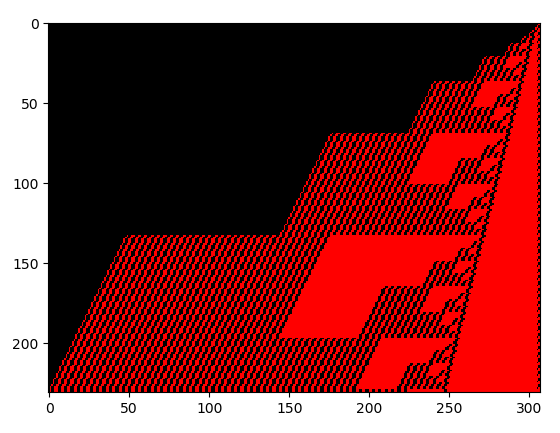
\includegraphics[width=0.45\textwidth]{16.png}
\label{fig:16}
\end{subfigure}
\hfill
\begin{subfigure}
\centering
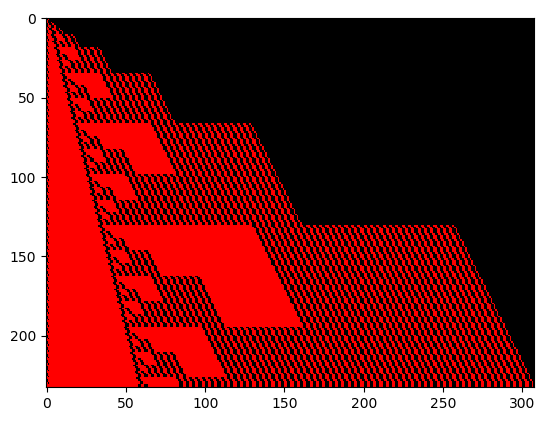
\includegraphics[width=0.45\textwidth]{24.png}
\label{fig:24}
\end{subfigure}
\caption{HNRs \#16 \& 24, tape head at extreme for up to 30000 steps.}
\end{figure}

\begin{figure}[H]
\centering
\begin{subfigure}
\centering
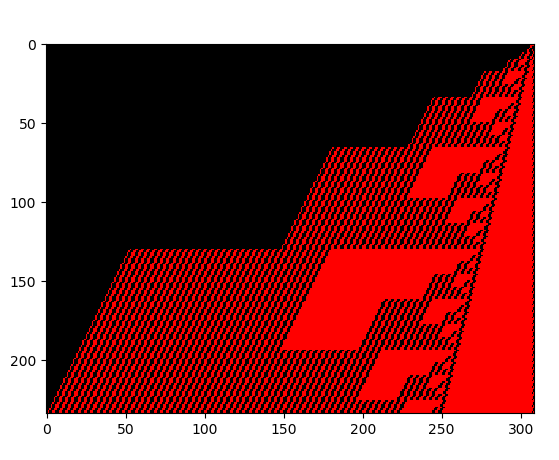
\includegraphics[width=0.45\textwidth]{38-r.png}
\label{fig:38r}
\end{subfigure}
\hfill
\begin{subfigure}
\centering
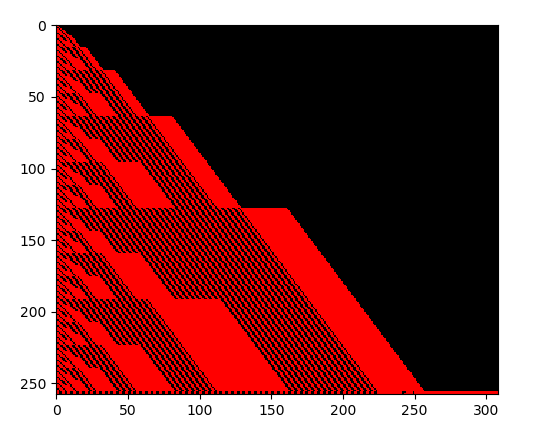
\includegraphics[width=0.45\textwidth]{38.png}
\label{fig:38l}
\end{subfigure}
\caption{HNR \#38, head at right, left resp. These three machines require but a routine proof.}
\end{figure}




\newpage
\addcontentsline{toc}{section}{17}
\section*{17}



\begin{table}[H]
\begin{Parallel}[c]{0.48\textwidth}{0.48\textwidth}
\ParallelLText{
\texttt{
\begin{scriptsize}
\begin{tabular}{rrl}
0&A&$o$\\
2&C&$i$\\
18&B&$(10)^{1}1i$\\
34&C&$(10)^{2}i$\\
66&B&$(10)^{1}1(10)^{1}1i$\\
88&D&$(10)^{2}1(10)^{1}i$\\
89&B&$(10)^{2}1(10)^{1}1o$\\
90&C&$(10)^{2}1(10)^{2}o$\\
91&D&$(10)^{2}1(10)^{2}0o$\\
95&C&$(10)^{2}1(10)^{2}1i$\\
219&C&$(10)^{4}1(10)^{2}1i$\\
335&B&$(10)^{4}1(10)^{2}1(10)^{1}1i$\\
451&C&$(10)^{4}1(10)^{2}1(10)^{2}i$\\
583&B&$(10)^{4}1(10)^{4}1(10)^{1}1i$\\
723&C&$(10)^{6}1(10)^{2}1(10)^{2}i$\\
895&B&$(10)^{1}1(10)^{4}1(10)^{4}1(10)^{1}1i$\\
1111&C&$(10)^{8}1(10)^{2}1(10)^{2}i$\\
1323&B&$(10)^{3}1(10)^{4}1(10)^{4}1(10)^{1}1i$\\
1675&C&$(10)^{8}1(10)^{4}1(10)^{2}i$\\
1911&B&$(10)^{3}1(10)^{6}1(10)^{4}1(10)^{1}1i$\\
2335&C&$(10)^{1}1(10)^{8}1(10)^{4}1(10)^{2}i$\\
2679&B&$(10)^{3}1(10)^{8}1(10)^{4}1(10)^{1}1i$\\
3175&C&$(10)^{3}1(10)^{8}1(10)^{4}1(10)^{2}i$\\
3687&B&$(10)^{3}1(10)^{8}1(10)^{6}1(10)^{1}1i$\\
4223&C&$(10)^{3}1(10)^{10}1(10)^{4}1(10)^{2}i$\\
4807&B&$(10)^{5}1(10)^{8}1(10)^{6}1(10)^{1}1i$\\
5507&C&$(10)^{3}1(10)^{12}1(10)^{4}1(10)^{2}i$\\
6163&B&$(10)^{7}1(10)^{8}1(10)^{6}1(10)^{1}1i$\\
6545&D&$(10)^{12}1(10)^{8}1(10)^{2}1(10)^{1}i$\\
6546&B&$(10)^{12}1(10)^{8}1(10)^{2}1(10)^{1}1o$\\
6547&C&$(10)^{12}1(10)^{8}1(10)^{2}1(10)^{2}o$\\
6548&D&$(10)^{12}1(10)^{8}1(10)^{2}1(10)^{2}0o$\\
6552&C&$(10)^{12}1(10)^{8}1(10)^{2}1(10)^{2}1i$\\
8200&C&$(10)^{12}1(10)^{8}1(10)^{4}1(10)^{2}1i$\\
9944&C&$(10)^{14}1(10)^{8}1(10)^{4}1(10)^{2}1i$\\
11988&C&$(10)^{16}1(10)^{8}1(10)^{4}1(10)^{2}1i$\\
13212&B&$(10)^{16}1(10)^{8}1(10)^{4}1(10)^{2}1(10)^{1}1i$\\
14436&C&$(10)^{16}1(10)^{8}1(10)^{4}1(10)^{2}1(10)^{2}i$\\
15676&B&$(10)^{16}1(10)^{8}1(10)^{4}1(10)^{4}1(10)^{1}1i$\\
16924&C&$(10)^{16}1(10)^{8}1(10)^{6}1(10)^{2}1(10)^{2}i$\\
18204&B&$(10)^{16}1(10)^{10}1(10)^{4}1(10)^{4}1(10)^{1}1i$\\
19524&C&$(10)^{18}1(10)^{8}1(10)^{6}1(10)^{2}1(10)^{2}i$\\
20940&B&$(10)^{1}1(10)^{16}1(10)^{10}1(10)^{4}1(10)^{4}1(10)^{1}1i$\\
22480&C&$(10)^{20}1(10)^{8}1(10)^{6}1(10)^{2}1(10)^{2}i$\\
\end{tabular}
\end{scriptsize}}}
\ParallelRText{
\texttt{
\begin{scriptsize}
\begin{tabular}{rrl}
24032&B&$(10)^{3}1(10)^{16}1(10)^{10}1(10)^{4}1(10)^{4}1(10)^{1}1i$\\
25876&C&$(10)^{20}1(10)^{10}1(10)^{6}1(10)^{2}1(10)^{2}i$\\
27500&B&$(10)^{3}1(10)^{18}1(10)^{10}1(10)^{4}1(10)^{4}1(10)^{1}1i$\\
29512&C&$(10)^{1}1(10)^{20}1(10)^{10}1(10)^{6}1(10)^{2}1(10)^{2}i$\\
31388&B&$(10)^{3}1(10)^{20}1(10)^{10}1(10)^{4}1(10)^{4}1(10)^{1}1i$\\
33568&C&$(10)^{3}1(10)^{20}1(10)^{10}1(10)^{6}1(10)^{2}1(10)^{2}i$\\
35780&B&$(10)^{3}1(10)^{20}1(10)^{12}1(10)^{4}1(10)^{4}1(10)^{1}1i$\\
38048&C&$(10)^{3}1(10)^{22}1(10)^{10}1(10)^{6}1(10)^{2}1(10)^{2}i$\\
40428&B&$(10)^{5}1(10)^{20}1(10)^{12}1(10)^{4}1(10)^{4}1(10)^{1}1i$\\
43004&C&$(10)^{3}1(10)^{24}1(10)^{10}1(10)^{6}1(10)^{2}1(10)^{2}i$\\
45552&B&$(10)^{7}1(10)^{20}1(10)^{12}1(10)^{4}1(10)^{4}1(10)^{1}1i$\\
48564&C&$(10)^{3}1(10)^{24}1(10)^{10}1(10)^{8}1(10)^{2}1(10)^{2}i$\\
51152&B&$(10)^{7}1(10)^{20}1(10)^{14}1(10)^{4}1(10)^{4}1(10)^{1}1i$\\
54268&C&$(10)^{3}1(10)^{26}1(10)^{10}1(10)^{8}1(10)^{2}1(10)^{2}i$\\
57024&B&$(10)^{9}1(10)^{20}1(10)^{14}1(10)^{4}1(10)^{4}1(10)^{1}1i$\\
60504&C&$(10)^{3}1(10)^{28}1(10)^{10}1(10)^{8}1(10)^{2}1(10)^{2}i$\\
63428&B&$(10)^{11}1(10)^{20}1(10)^{14}1(10)^{4}1(10)^{4}1(10)^{1}1i$\\
67396&C&$(10)^{3}1(10)^{28}1(10)^{12}1(10)^{8}1(10)^{2}1(10)^{2}i$\\
70408&B&$(10)^{11}1(10)^{22}1(10)^{14}1(10)^{4}1(10)^{4}1(10)^{1}1i$\\
74608&C&$(10)^{5}1(10)^{28}1(10)^{12}1(10)^{8}1(10)^{2}1(10)^{2}i$\\
77992&B&$(10)^{11}1(10)^{24}1(10)^{14}1(10)^{4}1(10)^{4}1(10)^{1}1i$\\
82424&C&$(10)^{7}1(10)^{28}1(10)^{12}1(10)^{8}1(10)^{2}1(10)^{2}i$\\
86340&B&$(10)^{11}1(10)^{24}1(10)^{14}1(10)^{6}1(10)^{4}1(10)^{1}1i$\\
90828&C&$(10)^{7}1(10)^{28}1(10)^{14}1(10)^{8}1(10)^{2}1(10)^{2}i$\\
94848&B&$(10)^{11}1(10)^{26}1(10)^{14}1(10)^{6}1(10)^{4}1(10)^{1}1i$\\
99568&C&$(10)^{9}1(10)^{28}1(10)^{14}1(10)^{8}1(10)^{2}1(10)^{2}i$\\
104016&B&$(10)^{11}1(10)^{28}1(10)^{14}1(10)^{6}1(10)^{4}1(10)^{1}1i$\\
108968&C&$(10)^{11}1(10)^{28}1(10)^{14}1(10)^{8}1(10)^{2}1(10)^{2}i$\\
113968&B&$(10)^{11}1(10)^{28}1(10)^{16}1(10)^{6}1(10)^{4}1(10)^{1}1i$\\
119040&C&$(10)^{11}1(10)^{30}1(10)^{14}1(10)^{8}1(10)^{2}1(10)^{2}i$\\
124272&B&$(10)^{13}1(10)^{28}1(10)^{16}1(10)^{6}1(10)^{4}1(10)^{1}1i$\\
129828&C&$(10)^{11}1(10)^{32}1(10)^{14}1(10)^{8}1(10)^{2}1(10)^{2}i$\\
135292&B&$(10)^{15}1(10)^{28}1(10)^{16}1(10)^{6}1(10)^{4}1(10)^{1}1i$\\
141552&C&$(10)^{11}1(10)^{32}1(10)^{14}1(10)^{8}1(10)^{4}1(10)^{2}i$\\
147040&B&$(10)^{15}1(10)^{28}1(10)^{16}1(10)^{8}1(10)^{4}1(10)^{1}1i$\\
153372&C&$(10)^{11}1(10)^{32}1(10)^{16}1(10)^{8}1(10)^{4}1(10)^{2}i$\\
158980&B&$(10)^{15}1(10)^{30}1(10)^{16}1(10)^{8}1(10)^{4}1(10)^{1}1i$\\
165576&C&$(10)^{13}1(10)^{32}1(10)^{16}1(10)^{8}1(10)^{4}1(10)^{2}i$\\
171700&B&$(10)^{15}1(10)^{32}1(10)^{16}1(10)^{8}1(10)^{4}1(10)^{1}1i$\\
178560&C&$(10)^{15}1(10)^{32}1(10)^{16}1(10)^{8}1(10)^{4}1(10)^{2}i$\\
185436&B&$(10)^{15}1(10)^{32}1(10)^{16}1(10)^{8}1(10)^{6}1(10)^{1}1i$\\
192336&C&$(10)^{15}1(10)^{32}1(10)^{16}1(10)^{10}1(10)^{4}1(10)^{2}i$\\
199284&B&$(10)^{15}1(10)^{32}1(10)^{18}1(10)^{8}1(10)^{6}1(10)^{1}1i$\\
206320&C&$(10)^{15}1(10)^{34}1(10)^{16}1(10)^{10}1(10)^{4}1(10)^{2}i$\\
213532&B&$(10)^{17}1(10)^{32}1(10)^{18}1(10)^{8}1(10)^{6}1(10)^{1}1i$\\
\end{tabular}
\end{scriptsize}}}
\end{Parallel}
\caption{\label{tab:17}Machine 17.}
\end{table}

\begin{table}[H]
\begin{Parallel}[c]{0.48\textwidth}{0.48\textwidth}
\ParallelLText{
\texttt{
\hspace*{-.5in}
\begin{tiny}
\begin{tabular}{rrl}
221140&C&$(10)^{15}1(10)^{36}1(10)^{16}1(10)^{10}1(10)^{4}1(10)^{2}i$\\
228616&B&$(10)^{19}1(10)^{32}1(10)^{18}1(10)^{8}1(10)^{6}1(10)^{1}1i$\\
236960&C&$(10)^{15}1(10)^{36}1(10)^{18}1(10)^{10}1(10)^{4}1(10)^{2}i$\\
244572&B&$(10)^{19}1(10)^{34}1(10)^{18}1(10)^{8}1(10)^{6}1(10)^{1}1i$\\
253212&C&$(10)^{17}1(10)^{36}1(10)^{18}1(10)^{10}1(10)^{4}1(10)^{2}i$\\
261428&B&$(10)^{19}1(10)^{36}1(10)^{18}1(10)^{8}1(10)^{6}1(10)^{1}1i$\\
270364&C&$(10)^{19}1(10)^{36}1(10)^{18}1(10)^{10}1(10)^{4}1(10)^{2}i$\\
279348&B&$(10)^{19}1(10)^{36}1(10)^{20}1(10)^{8}1(10)^{6}1(10)^{1}1i$\\
288436&C&$(10)^{19}1(10)^{38}1(10)^{18}1(10)^{10}1(10)^{4}1(10)^{2}i$\\
297716&B&$(10)^{21}1(10)^{36}1(10)^{20}1(10)^{8}1(10)^{6}1(10)^{1}1i$\\
307464&C&$(10)^{19}1(10)^{40}1(10)^{18}1(10)^{10}1(10)^{4}1(10)^{2}i$\\
317040&B&$(10)^{23}1(10)^{36}1(10)^{20}1(10)^{8}1(10)^{6}1(10)^{1}1i$\\
327696&C&$(10)^{19}1(10)^{40}1(10)^{18}1(10)^{12}1(10)^{4}1(10)^{2}i$\\
337344&B&$(10)^{23}1(10)^{36}1(10)^{22}1(10)^{8}1(10)^{6}1(10)^{1}1i$\\
348168&C&$(10)^{19}1(10)^{42}1(10)^{18}1(10)^{12}1(10)^{4}1(10)^{2}i$\\
358112&B&$(10)^{25}1(10)^{36}1(10)^{22}1(10)^{8}1(10)^{6}1(10)^{1}1i$\\
369652&C&$(10)^{19}1(10)^{44}1(10)^{18}1(10)^{12}1(10)^{4}1(10)^{2}i$\\
379892&B&$(10)^{27}1(10)^{36}1(10)^{22}1(10)^{8}1(10)^{6}1(10)^{1}1i$\\
392352&C&$(10)^{19}1(10)^{44}1(10)^{20}1(10)^{12}1(10)^{4}1(10)^{2}i$\\
402744&B&$(10)^{27}1(10)^{38}1(10)^{22}1(10)^{8}1(10)^{6}1(10)^{1}1i$\\
415564&C&$(10)^{21}1(10)^{44}1(10)^{20}1(10)^{12}1(10)^{4}1(10)^{2}i$\\
426680&B&$(10)^{27}1(10)^{40}1(10)^{22}1(10)^{8}1(10)^{6}1(10)^{1}1i$\\
439860&C&$(10)^{23}1(10)^{44}1(10)^{20}1(10)^{12}1(10)^{4}1(10)^{2}i$\\
451980&B&$(10)^{27}1(10)^{40}1(10)^{22}1(10)^{10}1(10)^{6}1(10)^{1}1i$\\
465248&C&$(10)^{23}1(10)^{44}1(10)^{22}1(10)^{12}1(10)^{4}1(10)^{2}i$\\
477536&B&$(10)^{27}1(10)^{42}1(10)^{22}1(10)^{10}1(10)^{6}1(10)^{1}1i$\\
491164&C&$(10)^{25}1(10)^{44}1(10)^{22}1(10)^{12}1(10)^{4}1(10)^{2}i$\\
504232&B&$(10)^{27}1(10)^{44}1(10)^{22}1(10)^{10}1(10)^{6}1(10)^{1}1i$\\
518220&C&$(10)^{27}1(10)^{44}1(10)^{22}1(10)^{12}1(10)^{4}1(10)^{2}i$\\
532272&B&$(10)^{27}1(10)^{44}1(10)^{24}1(10)^{10}1(10)^{6}1(10)^{1}1i$\\
546444&C&$(10)^{27}1(10)^{46}1(10)^{22}1(10)^{12}1(10)^{4}1(10)^{2}i$\\
560856&B&$(10)^{29}1(10)^{44}1(10)^{24}1(10)^{10}1(10)^{6}1(10)^{1}1i$\\
575864&C&$(10)^{27}1(10)^{48}1(10)^{22}1(10)^{12}1(10)^{4}1(10)^{2}i$\\
590636&B&$(10)^{31}1(10)^{44}1(10)^{24}1(10)^{10}1(10)^{6}1(10)^{1}1i$\\
597290&D&$(10)^{60}1(10)^{32}1(10)^{14}1(10)^{8}1(10)^{2}1(10)^{1}i$\\
597291&B&$(10)^{60}1(10)^{32}1(10)^{14}1(10)^{8}1(10)^{2}1(10)^{1}1o$\\
597292&C&$(10)^{60}1(10)^{32}1(10)^{14}1(10)^{8}1(10)^{2}1(10)^{2}o$\\
597293&D&$(10)^{60}1(10)^{32}1(10)^{14}1(10)^{8}1(10)^{2}1(10)^{2}0o$\\
597297&C&$(10)^{60}1(10)^{32}1(10)^{14}1(10)^{8}1(10)^{2}1(10)^{2}1i$\\
628321&C&$(10)^{60}1(10)^{32}1(10)^{14}1(10)^{8}1(10)^{4}1(10)^{2}1i$\\
659441&C&$(10)^{60}1(10)^{32}1(10)^{16}1(10)^{8}1(10)^{4}1(10)^{2}1i$\\
690945&C&$(10)^{62}1(10)^{32}1(10)^{16}1(10)^{8}1(10)^{4}1(10)^{2}1i$\\
723709&C&$(10)^{64}1(10)^{32}1(10)^{16}1(10)^{8}1(10)^{4}1(10)^{2}1i$\\
740873&B&$(10)^{64}1(10)^{32}1(10)^{16}1(10)^{8}1(10)^{4}1(10)^{2}1(10)^{1}1i$\\
758037&C&$(10)^{64}1(10)^{32}1(10)^{16}1(10)^{8}1(10)^{4}1(10)^{2}1(10)^{2}i$\\
775217&B&$(10)^{64}1(10)^{32}1(10)^{16}1(10)^{8}1(10)^{4}1(10)^{4}1(10)^{1}1i$\\
792405&C&$(10)^{64}1(10)^{32}1(10)^{16}1(10)^{8}1(10)^{6}1(10)^{2}1(10)^{2}i$\\
809625&B&$(10)^{64}1(10)^{32}1(10)^{16}1(10)^{10}1(10)^{4}1(10)^{4}1(10)^{1}1i$\\
826885&C&$(10)^{64}1(10)^{32}1(10)^{18}1(10)^{8}1(10)^{6}1(10)^{2}1(10)^{2}i$\\
844241&B&$(10)^{64}1(10)^{34}1(10)^{16}1(10)^{10}1(10)^{4}1(10)^{4}1(10)^{1}1i$\\
861765&C&$(10)^{66}1(10)^{32}1(10)^{18}1(10)^{8}1(10)^{6}1(10)^{2}1(10)^{2}i$\\
879641&B&$(10)^{1}1(10)^{64}1(10)^{34}1(10)^{16}1(10)^{10}1(10)^{4}1(10)^{4}1(10)^{1}1i$\\
897961&C&$(10)^{68}1(10)^{32}1(10)^{18}1(10)^{8}1(10)^{6}1(10)^{2}1(10)^{2}i$\\
916357&B&$(10)^{3}1(10)^{64}1(10)^{34}1(10)^{16}1(10)^{10}1(10)^{4}1(10)^{4}1(10)^{1}1i$\\
935653&C&$(10)^{68}1(10)^{34}1(10)^{18}1(10)^{8}1(10)^{6}1(10)^{2}1(10)^{2}i$\\
954313&B&$(10)^{3}1(10)^{66}1(10)^{34}1(10)^{16}1(10)^{10}1(10)^{4}1(10)^{4}1(10)^{1}1i$\\
974161&C&$(10)^{1}1(10)^{68}1(10)^{34}1(10)^{18}1(10)^{8}1(10)^{6}1(10)^{2}1(10)^{2}i$\\
993649&B&$(10)^{3}1(10)^{68}1(10)^{34}1(10)^{16}1(10)^{10}1(10)^{4}1(10)^{4}1(10)^{1}1i$\\
1014049&C&$(10)^{3}1(10)^{68}1(10)^{34}1(10)^{18}1(10)^{8}1(10)^{6}1(10)^{2}1(10)^{2}i$\\
1034545&B&$(10)^{3}1(10)^{68}1(10)^{36}1(10)^{16}1(10)^{10}1(10)^{4}1(10)^{4}1(10)^{1}1i$\\
1055225&C&$(10)^{3}1(10)^{70}1(10)^{34}1(10)^{18}1(10)^{8}1(10)^{6}1(10)^{2}1(10)^{2}i$
\end{tabular}
\end{tiny}}}
\ParallelRText{
\texttt{
\begin{tiny}
\begin{tabular}{rrl}
1076273&B&$(10)^{5}1(10)^{68}1(10)^{36}1(10)^{16}1(10)^{10}1(10)^{4}1(10)^{4}1(10)^{1}1i$\\
1097837&C&$(10)^{3}1(10)^{72}1(10)^{34}1(10)^{18}1(10)^{8}1(10)^{6}1(10)^{2}1(10)^{2}i$\\
1119437&B&$(10)^{7}1(10)^{68}1(10)^{36}1(10)^{16}1(10)^{10}1(10)^{4}1(10)^{4}1(10)^{1}1i$\\
1142157&C&$(10)^{3}1(10)^{72}1(10)^{34}1(10)^{20}1(10)^{8}1(10)^{6}1(10)^{2}1(10)^{2}i$\\
1163893&B&$(10)^{7}1(10)^{68}1(10)^{38}1(10)^{16}1(10)^{10}1(10)^{4}1(10)^{4}1(10)^{1}1i$\\
1186909&C&$(10)^{3}1(10)^{74}1(10)^{34}1(10)^{20}1(10)^{8}1(10)^{6}1(10)^{2}1(10)^{2}i$\\
1209197&B&$(10)^{9}1(10)^{68}1(10)^{38}1(10)^{16}1(10)^{10}1(10)^{4}1(10)^{4}1(10)^{1}1i$\\
1233153&C&$(10)^{3}1(10)^{76}1(10)^{34}1(10)^{20}1(10)^{8}1(10)^{6}1(10)^{2}1(10)^{2}i$\\
1255993&B&$(10)^{11}1(10)^{68}1(10)^{38}1(10)^{16}1(10)^{10}1(10)^{4}1(10)^{4}1(10)^{1}1i$\\
1281109&C&$(10)^{3}1(10)^{76}1(10)^{36}1(10)^{20}1(10)^{8}1(10)^{6}1(10)^{2}1(10)^{2}i$\\
1304229&B&$(10)^{11}1(10)^{70}1(10)^{38}1(10)^{16}1(10)^{10}1(10)^{4}1(10)^{4}1(10)^{1}1i$\\
1329961&C&$(10)^{5}1(10)^{76}1(10)^{36}1(10)^{20}1(10)^{8}1(10)^{6}1(10)^{2}1(10)^{2}i$\\
1354029&B&$(10)^{11}1(10)^{72}1(10)^{38}1(10)^{16}1(10)^{10}1(10)^{4}1(10)^{4}1(10)^{1}1i$\\
1380377&C&$(10)^{7}1(10)^{76}1(10)^{36}1(10)^{20}1(10)^{8}1(10)^{6}1(10)^{2}1(10)^{2}i$\\
1405697&B&$(10)^{11}1(10)^{72}1(10)^{38}1(10)^{18}1(10)^{10}1(10)^{4}1(10)^{4}1(10)^{1}1i$\\
1432197&C&$(10)^{7}1(10)^{76}1(10)^{38}1(10)^{20}1(10)^{8}1(10)^{6}1(10)^{2}1(10)^{2}i$\\
1457813&B&$(10)^{11}1(10)^{74}1(10)^{38}1(10)^{18}1(10)^{10}1(10)^{4}1(10)^{4}1(10)^{1}1i$\\
1484929&C&$(10)^{9}1(10)^{76}1(10)^{38}1(10)^{20}1(10)^{8}1(10)^{6}1(10)^{2}1(10)^{2}i$\\
1511549&B&$(10)^{11}1(10)^{76}1(10)^{38}1(10)^{18}1(10)^{10}1(10)^{4}1(10)^{4}1(10)^{1}1i$\\
1539281&C&$(10)^{11}1(10)^{76}1(10)^{38}1(10)^{20}1(10)^{8}1(10)^{6}1(10)^{2}1(10)^{2}i$\\
1567125&B&$(10)^{11}1(10)^{76}1(10)^{40}1(10)^{18}1(10)^{10}1(10)^{4}1(10)^{4}1(10)^{1}1i$\\
1595169&C&$(10)^{11}1(10)^{78}1(10)^{38}1(10)^{20}1(10)^{8}1(10)^{6}1(10)^{2}1(10)^{2}i$\\
1623629&B&$(10)^{13}1(10)^{76}1(10)^{40}1(10)^{18}1(10)^{10}1(10)^{4}1(10)^{4}1(10)^{1}1i$\\
1652733&C&$(10)^{11}1(10)^{80}1(10)^{38}1(10)^{20}1(10)^{8}1(10)^{6}1(10)^{2}1(10)^{2}i$\\
1681809&B&$(10)^{15}1(10)^{76}1(10)^{40}1(10)^{18}1(10)^{10}1(10)^{4}1(10)^{4}1(10)^{1}1i$\\
1712361&C&$(10)^{11}1(10)^{80}1(10)^{38}1(10)^{20}1(10)^{10}1(10)^{6}1(10)^{2}1(10)^{2}i$\\
1741509&B&$(10)^{15}1(10)^{76}1(10)^{40}1(10)^{20}1(10)^{10}1(10)^{4}1(10)^{4}1(10)^{1}1i$\\
1772229&C&$(10)^{11}1(10)^{80}1(10)^{40}1(10)^{20}1(10)^{10}1(10)^{6}1(10)^{2}1(10)^{2}i$\\
1801689&B&$(10)^{15}1(10)^{78}1(10)^{40}1(10)^{20}1(10)^{10}1(10)^{4}1(10)^{4}1(10)^{1}1i$\\
1833057&C&$(10)^{13}1(10)^{80}1(10)^{40}1(10)^{20}1(10)^{10}1(10)^{6}1(10)^{2}1(10)^{2}i$\\
1863609&B&$(10)^{15}1(10)^{80}1(10)^{40}1(10)^{20}1(10)^{10}1(10)^{4}1(10)^{4}1(10)^{1}1i$\\
1895625&C&$(10)^{15}1(10)^{80}1(10)^{40}1(10)^{20}1(10)^{10}1(10)^{6}1(10)^{2}1(10)^{2}i$\\
1927673&B&$(10)^{15}1(10)^{80}1(10)^{40}1(10)^{20}1(10)^{12}1(10)^{4}1(10)^{4}1(10)^{1}1i$\\
1959777&C&$(10)^{15}1(10)^{80}1(10)^{40}1(10)^{22}1(10)^{10}1(10)^{6}1(10)^{2}1(10)^{2}i$\\
1991993&B&$(10)^{15}1(10)^{80}1(10)^{42}1(10)^{20}1(10)^{12}1(10)^{4}1(10)^{4}1(10)^{1}1i$\\
2024425&C&$(10)^{15}1(10)^{82}1(10)^{40}1(10)^{22}1(10)^{10}1(10)^{6}1(10)^{2}1(10)^{2}i$\\
2057289&B&$(10)^{17}1(10)^{80}1(10)^{42}1(10)^{20}1(10)^{12}1(10)^{4}1(10)^{4}1(10)^{1}1i$\\
2090869&C&$(10)^{15}1(10)^{84}1(10)^{40}1(10)^{22}1(10)^{10}1(10)^{6}1(10)^{2}1(10)^{2}i$\\
2124381&B&$(10)^{19}1(10)^{80}1(10)^{42}1(10)^{20}1(10)^{12}1(10)^{4}1(10)^{4}1(10)^{1}1i$\\
2159369&C&$(10)^{15}1(10)^{84}1(10)^{42}1(10)^{22}1(10)^{10}1(10)^{6}1(10)^{2}1(10)^{2}i$\\
2193209&B&$(10)^{19}1(10)^{82}1(10)^{42}1(10)^{20}1(10)^{12}1(10)^{4}1(10)^{4}1(10)^{1}1i$\\
2228877&C&$(10)^{17}1(10)^{84}1(10)^{42}1(10)^{22}1(10)^{10}1(10)^{6}1(10)^{2}1(10)^{2}i$\\
2263897&B&$(10)^{19}1(10)^{84}1(10)^{42}1(10)^{20}1(10)^{12}1(10)^{4}1(10)^{4}1(10)^{1}1i$\\
2300245&C&$(10)^{19}1(10)^{84}1(10)^{42}1(10)^{22}1(10)^{10}1(10)^{6}1(10)^{2}1(10)^{2}i$\\
2336705&B&$(10)^{19}1(10)^{84}1(10)^{44}1(10)^{20}1(10)^{12}1(10)^{4}1(10)^{4}1(10)^{1}1i$\\
2373397&C&$(10)^{19}1(10)^{86}1(10)^{42}1(10)^{22}1(10)^{10}1(10)^{6}1(10)^{2}1(10)^{2}i$\\
2410537&B&$(10)^{21}1(10)^{84}1(10)^{44}1(10)^{20}1(10)^{12}1(10)^{4}1(10)^{4}1(10)^{1}1i$\\
2448465&C&$(10)^{19}1(10)^{88}1(10)^{42}1(10)^{22}1(10)^{10}1(10)^{6}1(10)^{2}1(10)^{2}i$\\
2486285&B&$(10)^{23}1(10)^{84}1(10)^{44}1(10)^{20}1(10)^{12}1(10)^{4}1(10)^{4}1(10)^{1}1i$\\
2525841&C&$(10)^{19}1(10)^{88}1(10)^{42}1(10)^{24}1(10)^{10}1(10)^{6}1(10)^{2}1(10)^{2}i$\\
2563829&B&$(10)^{23}1(10)^{84}1(10)^{46}1(10)^{20}1(10)^{12}1(10)^{4}1(10)^{4}1(10)^{1}1i$\\
2603745&C&$(10)^{19}1(10)^{90}1(10)^{42}1(10)^{24}1(10)^{10}1(10)^{6}1(10)^{2}1(10)^{2}i$\\
2642413&B&$(10)^{25}1(10)^{84}1(10)^{46}1(10)^{20}1(10)^{12}1(10)^{4}1(10)^{4}1(10)^{1}1i$\\
2683621&C&$(10)^{19}1(10)^{92}1(10)^{42}1(10)^{24}1(10)^{10}1(10)^{6}1(10)^{2}1(10)^{2}i$\\
2722969&B&$(10)^{27}1(10)^{84}1(10)^{46}1(10)^{20}1(10)^{12}1(10)^{4}1(10)^{4}1(10)^{1}1i$\\
2765769&C&$(10)^{19}1(10)^{92}1(10)^{44}1(10)^{24}1(10)^{10}1(10)^{6}1(10)^{2}1(10)^{2}i$\\
2805461&B&$(10)^{27}1(10)^{86}1(10)^{46}1(10)^{20}1(10)^{12}1(10)^{4}1(10)^{4}1(10)^{1}1i$\\
2849005&C&$(10)^{21}1(10)^{92}1(10)^{44}1(10)^{24}1(10)^{10}1(10)^{6}1(10)^{2}1(10)^{2}i$\\
2889997&B&$(10)^{27}1(10)^{88}1(10)^{46}1(10)^{20}1(10)^{12}1(10)^{4}1(10)^{4}1(10)^{1}1i$\\
2934285&C&$(10)^{23}1(10)^{92}1(10)^{44}1(10)^{24}1(10)^{10}1(10)^{6}1(10)^{2}1(10)^{2}i$\\
2977001&B&$(10)^{27}1(10)^{88}1(10)^{46}1(10)^{22}1(10)^{12}1(10)^{4}1(10)^{4}1(10)^{1}1i$\\
\end{tabular}
\end{tiny}}}
\end{Parallel}
\caption{\label{tab:17}Machine 17 continued.}
\end{table}

\newpage

\addcontentsline{toc}{section}{19$\sim$42}
\section*{19$\sim$42}

\begin{figure}[H]
\centering
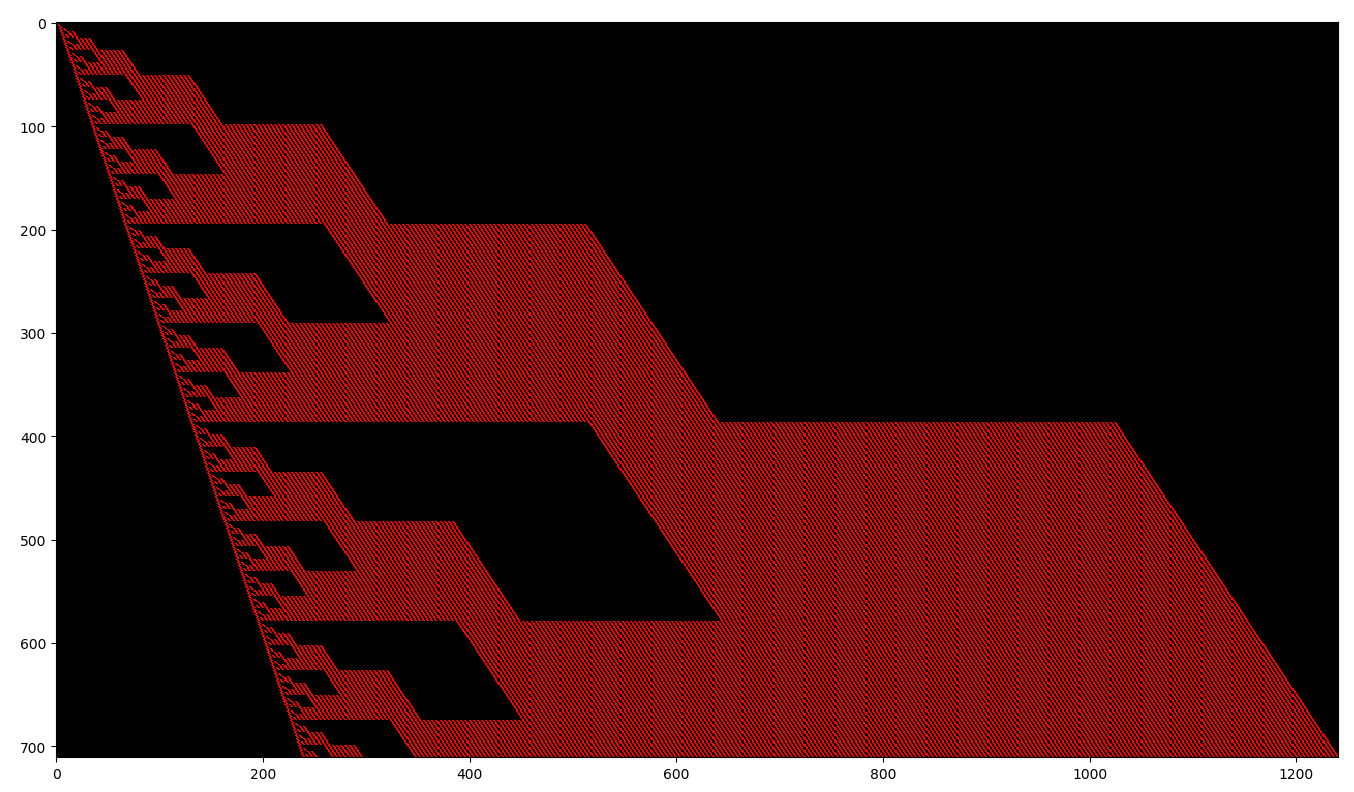
\includegraphics[width=0.8\textwidth]{19.png}
\caption{HNR \#19, tape head at left end for up to 300000 steps.}
\end{figure}

\begin{figure}[H]
\centering
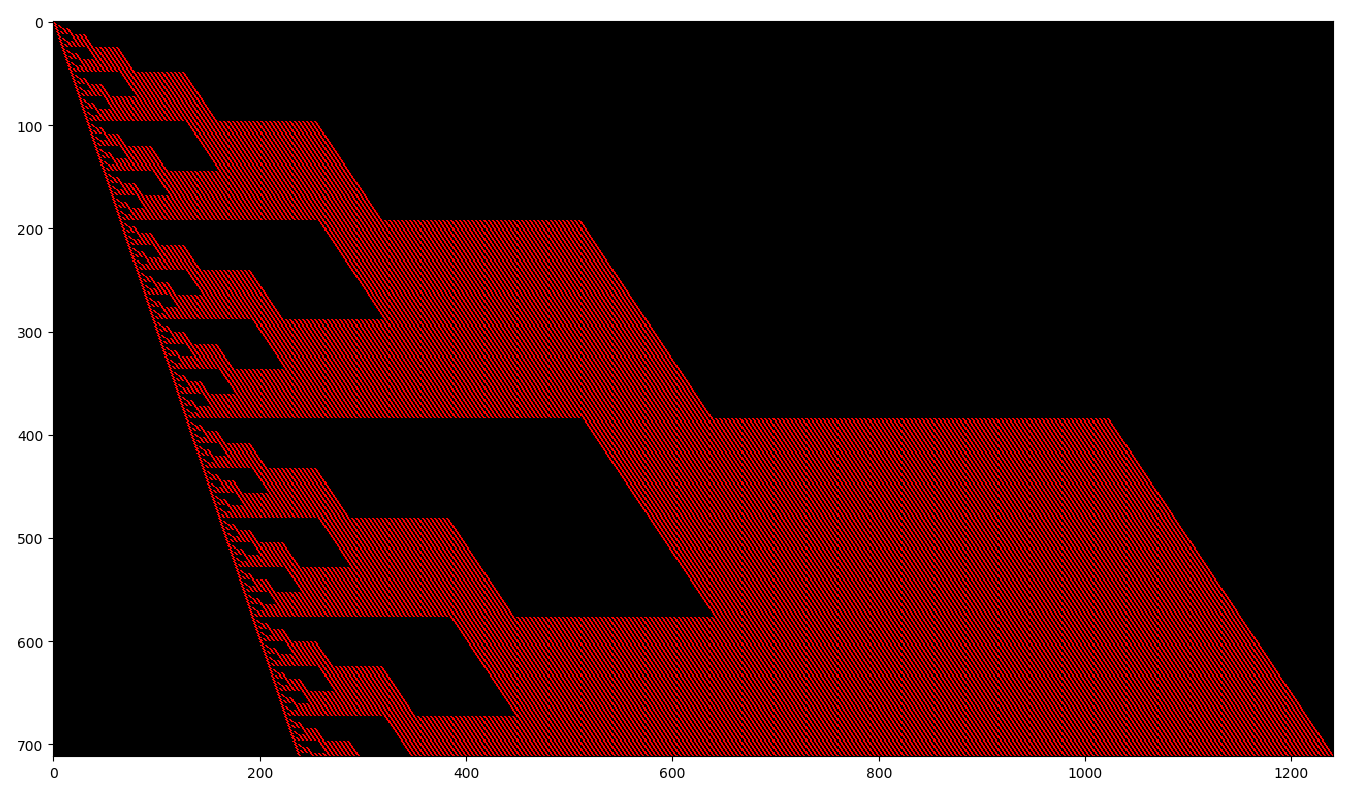
\includegraphics[width=0.8\textwidth]{42.png}
\caption{HNR \#42 similarly. These two require but a routine proof.}
\end{figure}


\addcontentsline{toc}{section}{20}
\section*{20}
Let
\begin{align*}
T &= 1001001000\\
U &= 10010010010101001101\\
V &= 1010011010\\
W &= 10011001001001010.\\
\end{align*}
Then we observe the following:
\begin{table}[H]
\texttt{
\begin{tabular}{rrl}
22613&E& $T^{09}V^{1.5}WU^{03.5}00i$\\
70779&E& $T^{16}V^{2.5}WU^{07.5}00i$\\
145633&E&$T^{23}V^{3.5}WU^{11.5}00i$\\
247175&E&$T^{30}V^{4.5}WU^{15.5}00i$\\
375405&E&$T^{37}V^{5.5}WU^{19.5}00i$\\
530323&E&$T^{44}V^{6.5}WU^{23.5}00i,$
\end{tabular}}
\end{table}
where the half-integer indicates an additional half a repetition.

So at intervals of $48166+26688k,$ the machine just adds seven $T$s, one $V$, and four $U$s.

So the proof for HNR\#20 will be easy if possibly arduous.

\newpage

\addcontentsline{toc}{section}{22}
\section*{22}
\newpage

\addcontentsline{toc}{section}{23=29}
\section*{23=29}

\begin{table}[H]
\texttt{
\begin{tabular}{rrl}
888&C&$(10)^{2}0(100)^{8}(10)^{7}i$\\
2820&C&$(10)^{2}0(100)^{18}(10)^{9}i$\\
7082&C&$(10)^{2}0(100)^{32}(10)^{11}i$\\
15114&C&$(10)^{2}0(100)^{50}(10)^{13}i$\\
28716&C&$(10)^{2}0(100)^{72}(10)^{15}i$\\
50048&C&$(10)^{2}0(100)^{98}(10)^{17}i$\\
81630&C&$(10)^{2}0(100)^{128}(10)^{19}i$\\
126342&C&$(10)^{2}0(100)^{162}(10)^{21}i$\\
187424&C&$(10)^{2}0(100)^{200}(10)^{23}i$
\end{tabular}}
\end{table}
The step differences are 1932, 4262, 8032, 13602, 21332, 31582, 44712, and 61082;\\
thus the second differences are 2330, 3770, 5570, 7730, 10250, 13130, and 16370,
the third differences are 1440, 1800, 2160, 2520, 2880, and 3240,
and the fourth differences are all 360.

So this machine will be fairly easy to prove never halts.

\newpage

\addcontentsline{toc}{section}{26}
\section*{26}
\begin{figure}[H]
\centering
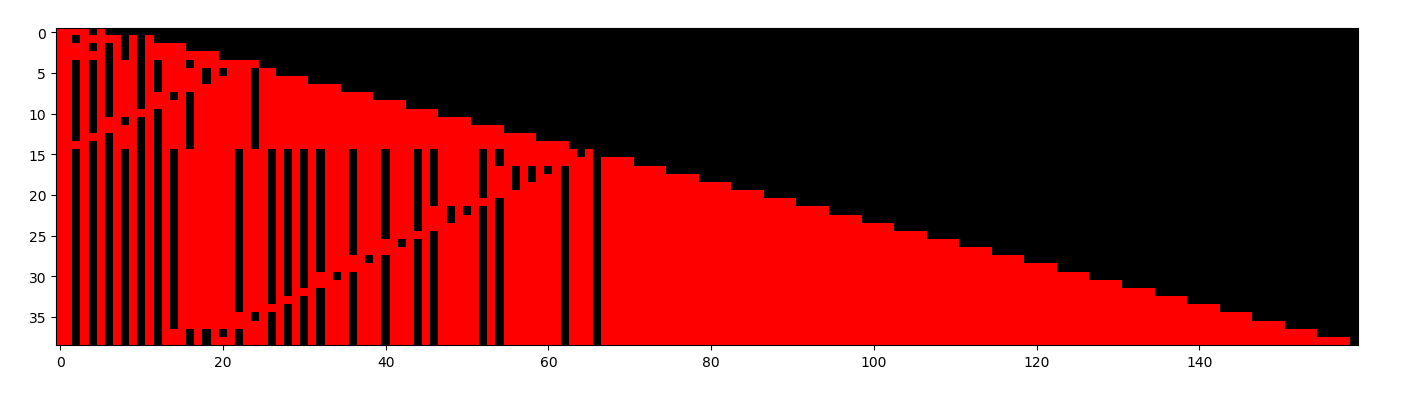
\includegraphics[width=\textwidth]{26.png}
\caption{HNR \#26, tape head at right end for 151029682 steps.\\
Each step number is roughly twice the previous.}
\end{figure}
The steps when HNR\#26 has reached the right end are 20, 84, 120, 184, 318, 343, 371, 435, 579, 859, 1431,
2583, 4879, 9483, 18695, 34848, 34858, 34902, 34966, 35102, 35382, 35954, 37110, 39406, 44006, 53218, 71650,
108506, 182234, 329682, 624594, 1214410, 2394054, 4753346, 9471934, 18909118, 37783478, 75532222, 151029686
shown in this picture. Denote this sequence by $a,$ and let $\Delta s$ denote the sequence $s_{i+1}-s_i$
for any sequence $s.$ Then it is observed that $\Delta a - \Delta^2 a$ is the sequence
92, 8, -6, 243, 22, -8, -16, 8, -12, -8, 8, -12, -4, 2271, 32296, -24, 24, -8, -8, -12, -12, 16, -8, -12,
-8, 8, -16, 8, -16, 8, -12, -4, -4, -8, 8, -24, 24.

In other words, the intervals between steps fail to double by very little in most transitions,
and where they fail greatly coordinates with the transition around the 15 mark in the picture.

\newpage

\addcontentsline{toc}{section}{BL\_2}
\section*{BL\_2}

\begin{table}[H]
\texttt{
\hspace*{-0.75in}
\begin{tabular}{rrl}
10&C&$i1011$\\
51&C&$i101(110)^{2}11$\\
214&C&$i101(110)^{1}1(110)^{5}11$\\
1063&C&$i101(110)^{1}1(110)^{2}10(110)^{12}11$\\
5834&C&$i101(110)^{1}1(110)^{2}10(110)^{2}1(110)^{32}11$\\
34397&C&$i101(110)^{1}1(110)^{2}10(110)^{2}1(110)^{6}1(110)^{80}11$\\
209800&C&$i101(110)^{1}1(110)^{2}10(110)^{2}1(110)^{6}1(110)^{14}1(110)^{200}11$\\
1298303&C&$i101(110)^{1}1(110)^{2}10(110)^{2}1(110)^{6}1(110)^{14}1(110)^{34}1(110)^{500}11$\\
8082056&C&$i101(110)^{1}1(110)^{2}10(110)^{2}1(110)^{6}1(110)^{14}1(110)^{34}1(110)^{84}1(110)^{1250}11$\\
50432059&C&$i101(110)^{1}1(110)^{2}10(110)^{2}1(110)^{6}1(110)^{14}1(110)^{34}1(110)^{84}1(110)^{209}1(110)^{3125}11$\\
315021908&C&$i101(110)^{1}1(110)^{2}10(110)^{2}1(110)^{6}1(110)^{14}1(110)^{34}1(110)^{84}1(110)^{209}1(110)^{522}10(110)^{7812}11$\\
\end{tabular}}
\end{table}
Let $a_i$ and $b_i$ denote the exponents of the last and second to last swath of 110s during a given step
when the tape head has reached the right edge of the tape anew, as written above.

Then it appears to be the case that
\begin{align*}
b_{i+1}&=\lceil a_i/6\rceil+t\\
a_{i+1}&=\lfloor5a_i/2\rfloor
\end{align*}
where $t$ is 1 if $a_i$ is $5\pmod6$ and 0 otherwise.

Although it is too early to tell, it seems likely that HNR\#BL_2 will not be very difficult.
\newpage

\addcontentsline{toc}{section}{30=41}
\section*{30=41}
\addcontentsline{toc}{section}{33}
\section*{33}
\addcontentsline{toc}{section}{34}
\section*{34}
\addcontentsline{toc}{section}{35}
\section*{35}
\addcontentsline{toc}{section}{36}
\section*{36}
\addcontentsline{toc}{section}{37}
\section*{37}
\addcontentsline{toc}{section}{40}
\section*{40}
\addcontentsline{toc}{section}{43}
\section*{43}

\end{document}